\documentclass{article}

\usepackage{graphicx}
\usepackage[utf8]{inputenc}
\usepackage[english]{babel}
\usepackage[document]{ragged2e}
\usepackage{geometry}
 \geometry{
 a4paper,
 total={170mm,257mm},
 left=20mm,
 top=20mm,
 }


\begin{document}
{\textbf{CS663: Assignment 4 - Q2}}
\vskip 0.2in

Pranav Sankhe \\ Kalpesh Krishna \\ Mohit Madan 

\vskip 0.5in
Q. Reconstruction of any one face image from the training dataset and visualization of first 25 eigenfaces. 

\vskip 0.2in

\textbf{Results}

\vskip 0.5in
Reconstruction of an image for various value of principal components. 
k = [2 10 20 50 75 100 125 150 175] 
The 1st image corresponds to the \texttt{k = 1} and lastimage coresponds to \texttt{k = 170} and the inbetween images are arranged accordingly. 

We can also see from the results that how PCA can be implemented for denoising of an image.

\begin{figure}[h!]
  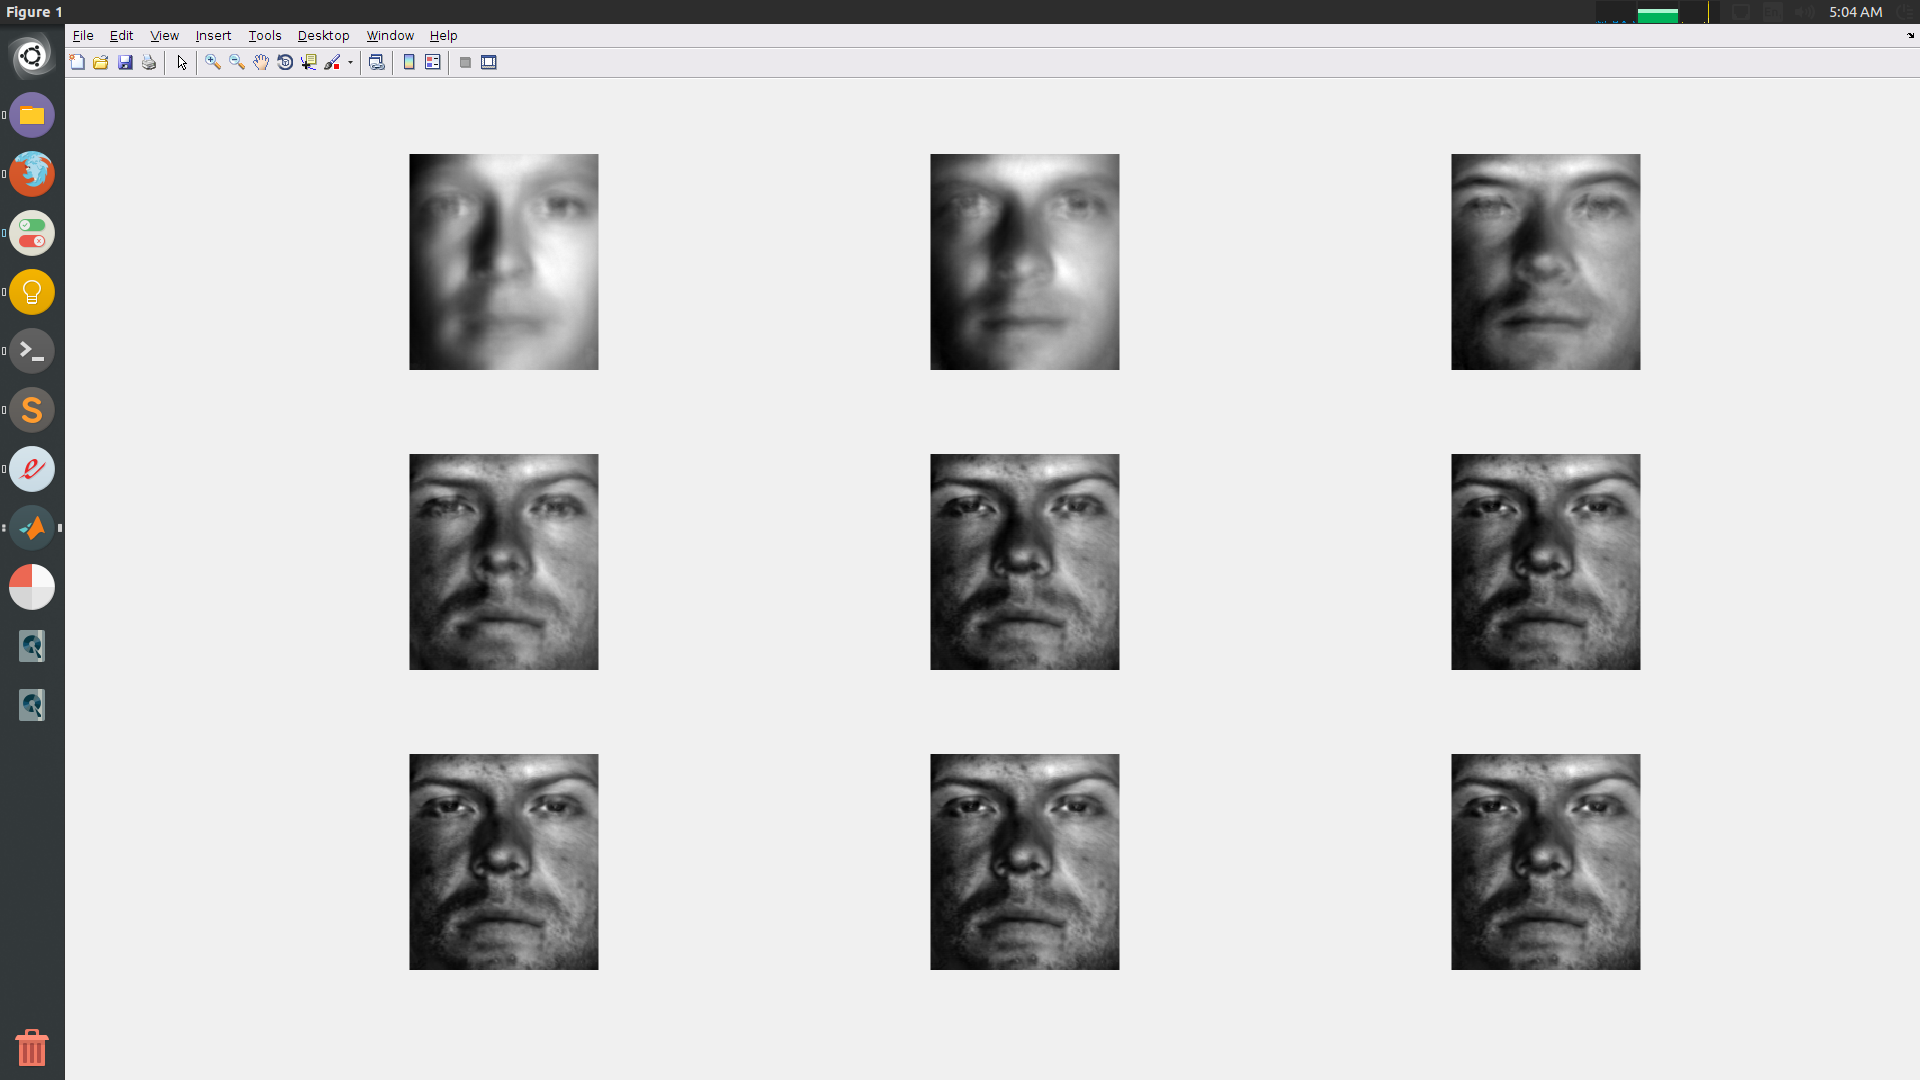
\includegraphics[width=\linewidth]{recon.png}
  \caption{Reconstructed image for various value of principal components)}
  \label{fig:result1}
\end{figure}
\newpage
Top 25 eigenfaces
\begin{figure}[h!]
  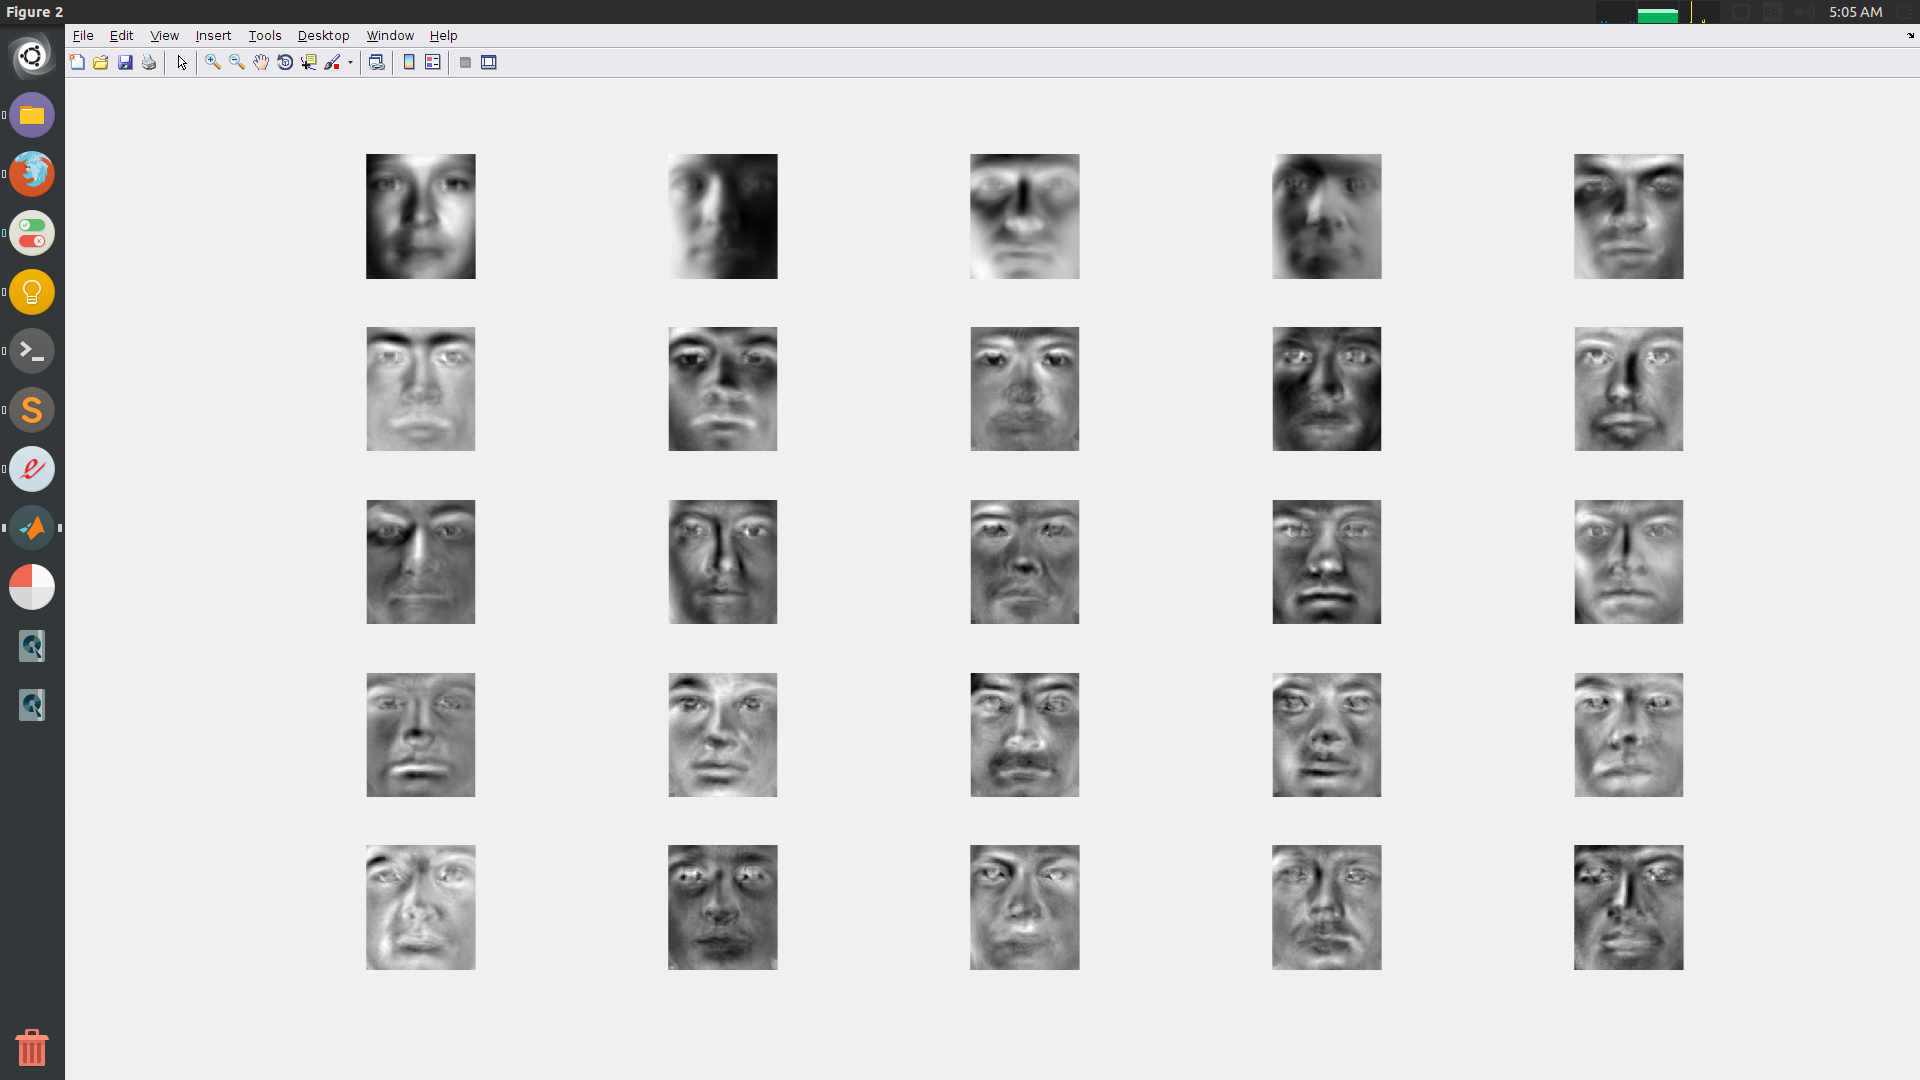
\includegraphics[width=\linewidth]{first_25.png}
  \caption{first 25 eigenfaces}
  \label{fig:result2}
\end{figure}

\textbf{Note:} All the datasets directories were in the main folder of the assignement alongside the folders of individual questions. 


\end{document}